% !TEX root = ../main.tex

\section{Introduction}

Consider Alice, a trader who wants to buy 100 shares of AAPL (Apple) on Nasdaq during regular trading hours. She can choose from dozens of order types and configurations, but her order ultimately gets submitted to one of Nasdaq's two main trading systems, each with a distinct \textit{market design}: AAPL's continuous limit order book (CLOB) or its closing cross (a type of call market)~\cite{Har03}. An order submitted to the CLOB can execute as soon as a compatible order is available. In contrast, an order submitted to the closing cross is held until the end of the trading day, when buy and sell orders are matched simultaneously at a single price that maximizes the number of shares traded. This price becomes AAPL's official closing price. 

Most trading occurs through the CLOB, but the closing cross is particularly important to institutional investors, such as mutual funds and index funds. These investors often need to buy or sell large quantities of shares at a fair and predictable price. By collecting orders and executing them together at a single price, the closing cross helps reduce the impact of large trades on the market and provides a common price against which investors can measure their performance.

One concern for traders is high-frequency trading (HFT), where specialized firms use sophisticated technology to place and execute orders faster than other traders, sometimes gaining an unfair advantage. This is particularly problematic in the CLOB, where orders execute continuously and even a tiny speed advantage can make a difference. In contrast, the closing cross executes orders together at a single price, making the advantage of being faster than other traders negligible. If Alice wants to avoid competing with HFTs, she could submit her order to the closing cross. However, she would have to wait until the end of the trading day, without knowing the exact price she will pay or even whether her order will execute. 

\paragraph{Frequent batch auctions (FBAs).} FBAs have been proposed as a middle ground between these two market designs~\cite{BCS15}. Rather than matching orders continuously or only at the end of the day, FBAs collect orders over short intervals (e.g., 100 milliseconds) and execute them together at a single price. This allows Alice to trade throughout the day while making the speed advantages exploited by HFTs largely irrelevant. Variants of FBAs have already been deployed in practice: Cboe~\cite{+cboefba} introduced periodic auctions in European equity markets in 2015 and U.S. equity markets in 2022, allowing traders to participate in short, order-triggered auctions throughout the trading day.

\paragraph{Transparency of FBAs.} One drawback of FBAs compared to CLOBs is their limited transparency, a distinction examined by the European Securities and Markets Authority (ESMA)~\cite{+esmafba,+esmafbafinal}. In a CLOB, the publicly displayed order book is visible to traders. Alice cannot know what other orders will arrive before hers, or how the book will change before her order executes. Furthermore, some orders may be hidden. Nevertheless, the visible order book and trading history provide information that Alice can use to assess why her order executed, remained unfilled, or executed at a particular price.

FBAs are different. Orders are collected over a short time window and executed together when the auction closes. During this interval, Alice may see an indicative clearing price and volume, but not the individual orders that determine them. Even after the auction closes, she typically sees the outcome rather than the full set of submitted orders, including those that did not execute but may have influenced the clearing price. Consequently, Alice cannot independently verify that the exchange included all eligible orders, excluded ineligible ones, calculated the correct clearing price, and allocated trades according to the rules. This limited transparency is partly intentional: revealing pending orders could expose traders to front-running and other forms of exploitation.

\paragraph{Zero-Knowledge Proofs (ZKPs).} ZKPs offer a way to address the transparency problem without revealing traders' private orders. We develop a zero-knowledge frequent batch auction (zk-FBA) protocol in which the exchange publishes the auction outcome alongside a proof proving that the clearing price and allocation were computed correctly from the submitted orders. Specifically, we make the following contributions:

\begin{itemize}
\item We design a zk-FBA protocol that supports common order types and proves the correctness of market clearing and the quantities needed to calculate individual trade allocations, without revealing private orders.
\item We develop an application-specific arithmetization of the market clearing algorithm within the polynomial interactive oracle proof (PIOP) model for zk-SNARKs, optimizing for fast proof generation while retaining a small, constant-size clearing proof with short verification time independent of the number of orders.
\item As a side-product, we also develop reusable gadgets for efficiently proving minimum, maximum, and absolute-value relationships over private values. 
\item We implement the protocol and benchmark its performance across different auction sizes, measuring proof generation time, verification time, and proof size.\footnote{GitHub: \anonalt{\url{https://github.com/MadibaGroup/2024-zkFBA}}{https://anonymous.4open.science/r/DeFi2027-4672/README.md}}
\end{itemize}

\paragraph{Relevance to decentralized finance (DeFi).} Our contributions provide a building block for verifiable trading across different market structures. In DeFi, a smart contract could collect orders and verify a clearing proof on-chain before settling trades (\cf~\cite{GY21,MoCl23}). A hybrid DEX could instead collect orders privately off-chain, while using the proof for on-chain settlement. Traditional exchanges could also adopt zk-FBA, or use our techniques to verify opening and closing auctions without changing their continuous trading mechanisms (\eg NYSE, Nasdaq).
% = = = = = = = = = 

\section{Background}

\paragraph{Related Work.} Budish, Cramton, and Shim popularized FBAs as an alternative to CLOBs to reduce the speed advantages of HFTs~\cite{BCS15}. That said, earlier trading systems employed similar designs without using the term FBA. One example from traditional markets is the now-defunct OptiMark trading system, launched in 1999, which used 90-second auctions to match complex trading orders~\cite{CW01}. Another example from decentralized finance (DeFi) was the ``Princeton'' prediction market~\cite{BCFKMN14}, which proposed having miners run a batch auction every block (approximately every 10 minutes) to mitigate front-running attacks, now recognized as a form of maximal extractable value (MEV).

Zero-knowledge proofs have previously been applied to verifiable auctions~\cite{PRST06}, including periodic auctions~\cite{GY21}, using Zokrates, a high-level ZKP language. On-chain blockchain-based batch auctions~\cite{MDFO22,MoCl23} use FBAs to mitigate MEV, while others propose hybrid designs~\cite{CC22}.

Improving prover time in zk-SNARKs through \textit{\ari} has been explored in other applications, including electronic voting~\cite{MEC26} and proofs of solvency~\cite{DC26}. Rather than expressing the computation as a general-purpose arithmetic circuit or zkVM program, custom arithmetization encodes the application directly into the polynomial constraints of the SNARK. The resulting zk-SNARK is specialized for that particular computation, sacrificing generality in exchange for faster proof generation.

Unlike the closest prior art~\cite{GY21}, our protocol is designed for FBAs, supporting the three principal order types used in NASDAQ's Closing Cross: market-on-close, limit-on-close, and imbalance-only orders. By encoding the clearing and allocation rules directly into the arithmetization, we optimize proof generation for frequent auction clearing.

\paragraph{Batch Auctions.} The NYSE and NASDAQ use batch auctions before trading hours to set opening prices and at the end of trading hours to set closing prices. They are also known as call markets or crosses. An FBA runs such a market frequently during the day, such as every 1 s or 100 ms. Alternatively, an auction may be triggered by the arrival of orders (\eg Cboe US). Orders are matched at a single clearing price chosen to maximize executable volume, with further rules based on order imbalance to resolve ties. Depending on the available liquidity and the allocation rules, eligible orders may be fully executed, partially filled, or left unfilled.

Batch auctions support several order types, which can be further configured with additional instructions. We consider three types, using the terminology established for orders submitted to the closing market (``on-close'' orders), although our FBAs need not occur at market close. A limit-on-close (LOC) order specifies a side (buy or sell), a price, and a volume. A buy LOC is eligible to execute at or below its limit price, while a sell LOC is eligible at or above its limit. A market-on-close (MOC) order specifies a side and volume but no price, and is eligible to execute at the clearing price. An imbalance-only (IO) order specifies a side, price, and volume, but executes only if it offsets an imbalance between ordinary buy and sell orders. IO orders do not influence the clearing price and appeal to traders who want to execute large trades slowly with no price impact. %Appendix~\ref{sec:market-close} describes the clearing algorithm we will prove.

At the close of each batch, the exchange publishes either a \textsc{No-Cross} outcome or a \emph{clearing receipt}. The receipt contains the market-clearing price and maximum executable volume, together with the interval of prices attaining that maximum, the remaining order imbalance and its side, and quantities needed to determine partial fills. Traders use this public information, together with their own orders, to check that their trade executions match. The underlying order book remains private from the public.

% = = = = = = = = = 
\begin{figure}[!tp]
    \centering
    \adjustbox{angle=90,max totalsize={\linewidth}{0.85\textheight}}{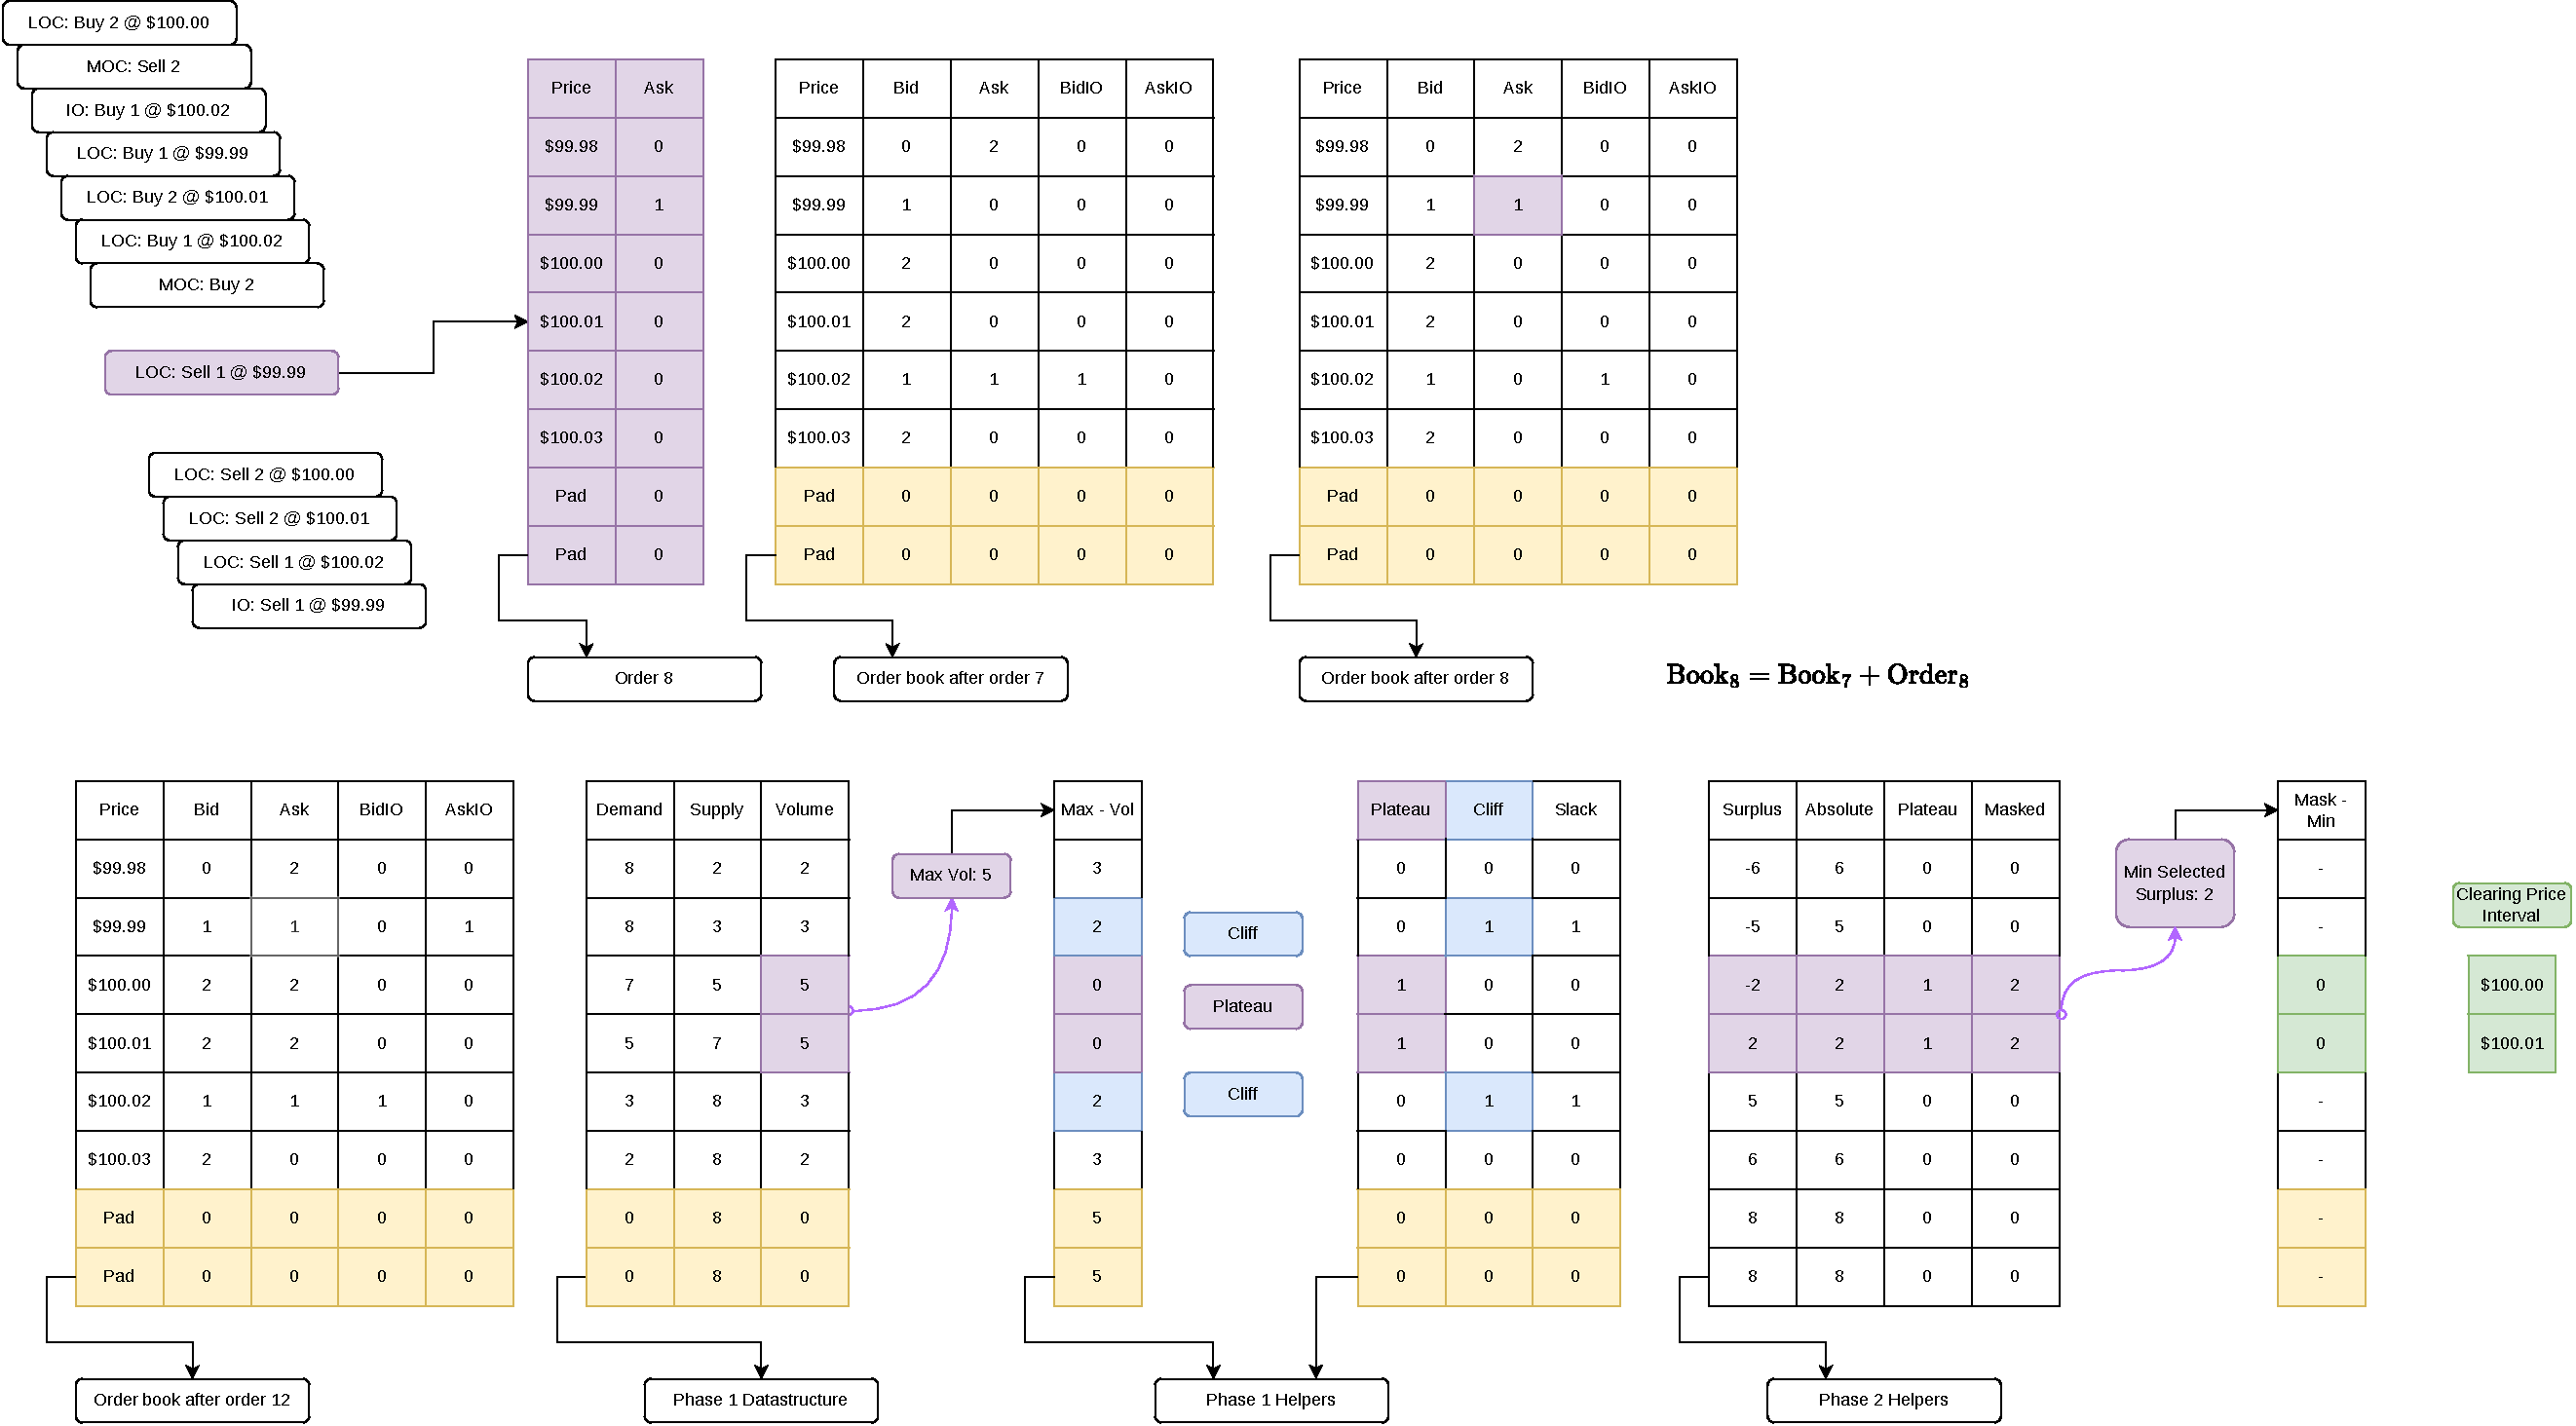
\includegraphics{figures/overview.pdf}}
    \caption{Overview of the batch-auction example. \textbf{Top:} Sequential order submissions update the aggregated order book, illustrated by the eighth order. \textbf{Bottom:} The clearing algorithm maximizes executable volume (Phase 1) and minimizes imbalance (Phase 2), using auxiliary columns to certify the results. Six price ticks are padded to eight rows. Phase 3 (not shown) selects a single clearing price, admits eligible IO orders, and determines execution quantities and partial-fill ratios.}
    \label{fig:overview}
\end{figure}
% = = = = = = = = = 

\section{Arithmetization of Market Clearing}
\label{sec:clearing-constraints}

Figure~\ref{fig:overview} illustrates a running example of market clearing. The top shows how orders are accumulated into an order book, while the bottom shows how the completed book is processed. We explain the bottom first, returning to order submission in Section~\ref{sec:order-receipts}. For now, we assume that the order book is complete and ready to be processed. The clearing algorithm examines the book and determines a single \emph{market-clearing price} at which all trades execute. For example, Alice might submit a bid of \$100.02 but execute at \$100.00, receiving a \emph{price improvement}. However, even at the clearing price, there may be more demand than supply (or vice versa), meaning some eligible orders cannot be filled completely. The algorithm seeks to maximize executable volume and minimize the remaining imbalance, with IO orders providing additional liquidity. Any remaining excess must be rationed among eligible orders, potentially through pro-rata partial fills.

Arithmetization is the process of expressing a computation as polynomial constraints that a zero-knowledge proof system can verify. Polynomial interactive oracle proof (PIOP)-based zk-SNARKs, such as PLONK and its many variants~~\cite{GWC19,CBBZ23}, arithmetize a general-purpose circuit or a virtual machine (VM) execution trace. For example, for comparison, we implement the market-clearing algorithm in Noir, which compiles it into polynomial constraints. However the overhead-reducing approach is \textit{\ari}, which means working directly at the arithmetization level, expressing the algorithm as polynomial relationships without first implementing it as a circuit.

Developing \ari is not automated: it requires understanding both the mathematical structure of the algorithm and the available constraint gadgets, then identifying how they fit together. The algorithm must have enough exploitable structure to be expressed efficiently using operations such as addition, multiplication, equality checks, recurrences, and range checks. Where existing gadgets are insufficient, new ones may be developed---for example, we construct specialized gadgets for minimum, maximum, and absolute value. By exploiting the structure of market clearing, our custom arithmetization achieves faster proof generation than the Noir implementation, as demonstrated in our evaluation.


\subsection{From Algorithm to Polynomial Constraints}

\begin{figure}[t]
\centering
% !TEX root = ../main.tex



\begin{minipage}[t]{0.48\linewidth}
\textbf{(a) Algorithm}\par\smallskip
\begin{adjustbox}{max width=\linewidth}
\begin{minipage}{\textwidth}
\begin{algorithmic}[1]
\For{$i=0,\ldots,N-1$}
    \State $AccB_i \gets \sum_{j=i}^{N-1} B_j$
    \State $AccA_i \gets \sum_{j=0}^{i} A_j$
    \State \mbox{$Min_i \gets \min\{AccB_i,AccA_i\}$}
\EndFor
\end{algorithmic}
\end{minipage}
\end{adjustbox}
\end{minipage}
\hfill
\begin{minipage}[t]{0.48\linewidth}
\textbf{(b) Recurrences}\par\smallskip
\begin{adjustbox}{max width=\linewidth}
\begin{minipage}{\textwidth}
\begin{algorithmic}[1]
\State $AccB_{N-1} \gets B_{N-1}$
\For{$i=N-2,\ldots,0$}
    \State $AccB_i \gets B_i+AccB_{i+1}$
\EndFor
\State $AccA_0 \gets A_0$
\For{$i=1,\ldots,N-1$}
    \State $AccA_i \gets A_i+AccA_{i-1}$
\EndFor
\For{$i=0,\ldots,N-1$}
    \State \mbox{$Min_i \gets \min\{AccB_i,AccA_i\}$}
\EndFor
\end{algorithmic}
\end{minipage}
\end{adjustbox}
\end{minipage}

\medskip

\begin{minipage}[t]{0.48\linewidth}
\textbf{(c) Polynomial evaluations}\par\smallskip
\begin{adjustbox}{max width=\linewidth}
$\displaystyle
\begin{aligned}
AccB(\omega^i) &= B(\omega^i)+AccB(\omega^{i+1})\\
AccA(\omega^{i+1}) &= AccA(\omega^i)+A(\omega^{i+1})\\
Min(\omega^i) &= \min\{AccB(\omega^i),AccA(\omega^i)\}
\end{aligned}
$
\end{adjustbox}
\end{minipage}
\hfill
\begin{minipage}[t]{0.48\linewidth}
\textbf{(d) Polynomial constraints}\par\smallskip
\begin{adjustbox}{max width=\linewidth}
$\displaystyle
\begin{aligned}
\mathrm{F5:}\quad &L_{n-1}(X)(AccB(X)-B(X))=0\\
\mathrm{F6:}\quad &L_0(X)(AccA(X)-A(X))=0\\
\mathrm{F7:}\quad &(X-\omega^{n-1})(AccB(X)-AccB(\omega X)-B(X))=0\\
\mathrm{F8:}\quad &(X-\omega^{n-1})(AccA(\omega X)-AccA(X)-A(\omega X))=0\\
\mathrm{F9:}\quad &SurpB(X)=AccB(X)-Min(X)\\
\mathrm{F10:}\quad &SurpA(X)=AccA(X)-Min(X)\\
\mathrm{F11:}\quad &SurpA(X)\cdot SurpB(X)=0\\
\mathrm{F12:}\quad &SurpB_i\in[0,2^k)\\
\mathrm{F13:}\quad &SurpA_i\in[0,2^k)
\end{aligned}
$
\end{adjustbox}
\end{minipage}


\caption{Four stages of arithmetizing executable volume: (a) the original computation, (b) an equivalent recurrence formulation, (c) the recurrences expressed as polynomial evaluations, and (d) polynomial constraints that enforce the computation, including boundary conditions and a minimum gadget. The F-numbers refer to the complete constraint system below.}
\label{fig:arithmetization}
\end{figure}

To illustrate our arithmetization technique, we focus on one part of market clearing: calculating how many shares can be traded at each possible price. Figure~\ref{fig:arithmetization} presents four representations of this computation, moving from a conventional algorithm to polynomial constraints. This example introduces the main techniques only, as we do not have space to explain every constraint presented in Section~\ref{sec:constraints}.

Like other \ari protocols, we use a set of one-dimensional arrays (\aka vectors or columns in Figure~\ref{fig:overview}) as our basic data structure. We decide to encode prices by having each index $i$ corresponds to a possible trading price $\pi_i$. This mapping between indices and prices is public and is not stored in the proof anywhere. This means that an output such as a market clearing price is not expressed as a dollar amount, it is expressed as an index. Outside of the proof, the index is mapped to a price. This representation has one drawback: the exchange must anticipate a sufficiently wide range of trading prices. A wider range increases computational costs, while a narrower range risks excluding prices at which traders wish to transact. We note without proof that the arrays can be extended at additional computational cost, preventing the exchange from becoming trapped within its initial price bounds.  In Figure~\ref{fig:overview}, six indices correspond to prices from \$99.98 to \$100.03, in one-cent increments.

Let $B$ and $A$ denote arrays containing the total buy and sell quantities, respectively. These are the columns marked ``Bid'' and ``Ask'' in the completed order book of Figure~\ref{fig:overview}. LOC orders are added at the index that corresponds to their limit price. MOC orders are placed at the highest price for buys and the lowest price for sells, ensuring they are eligible at every possible clearing price. IO orders are stored in separate arrays and considered only in Phase 3.

Figure~\ref{fig:arithmetization}(a) shows a straightforward computation of executable volume. At each price, cumulative demand includes all buy orders at that price or higher, while cumulative supply includes all sell orders at that price or lower. The executable volume is the smaller of these two quantities. In the figure, we use $AccB_i$, $AccA_i$, and $Min_i$ for these three values. In Figure~\ref{fig:overview}, demand at \$100.00 is 7 shares and supply is 5, giving an executable volume of 5. The maximum executable volume is 5, attained at both \$100.00 and \$100.01.

Our first transformation replaces cumulative sums with recurrences, as shown in Figure~\ref{fig:arithmetization}(b). Rather than summing over multiple entries at each price, demand and supply are calculated using their values at adjacent prices. This produces the same results while expressing the computation as local relationships, which are more convenient to enforce using polynomial constraints.

Next, we represent the arrays as evaluations of univariate polynomials. We first pad the arrays with zeros to a power-of-two length $n\geq N$. In Figure~\ref{fig:overview}, the six possible prices become eight rows. These extra rows do not represent additional prices; they accommodate the polynomial representation. Let $\mathbb{F}$ be a finite field and $H=\{1,\omega,\ldots,\omega^{n-1}\}$ an evaluation domain, where $\omega$ is a primitive $n$-th root of unity. Each array is represented by a polynomial whose evaluations at these points equal its entries. For example, $B(\omega^i)=B_i$, while $AccB(\omega^i)=AccB_i$.

The key observation is that moving from index $i$ to $i+1$ corresponds to replacing $\omega^i$ with $\omega^{i+1}$. Figure~\ref{fig:arithmetization}(c) expresses the recurrences in terms of polynomial evaluations. For example, $AccB(\omega^i)=B(\omega^i)+AccB(\omega^{i+1})$ is the polynomial representation of the demand recurrence. At \$100.00 in our example, this gives $7=2+5$. The minimum operation is also expressed in terms of polynomial evaluations, although it is not yet a polynomial constraint.

The final transformation, shown in Figure~\ref{fig:arithmetization}(d), constructs constraints that enforce these relationships. It is important to understand that constraints are not an algorithm to calculate results. The prover first runs the algorithm and generates all the intermediate and final values (the \emph{witness}). The prover knows that demand is 7 and supply is 5, and can assert that this true. The constraints then establish that this claim is correct.

Since $\omega^n=1$, advancing from the last evaluation point wraps around to the first. We therefore disable the recurrences at the final row and impose their boundary conditions separately. Let $L_i(X)$ denote the Lagrange polynomial that evaluates to 1 at row $i$ and 0 at every other row. Multiplying a constraint by $L_i(X)$ restricts it to that row, while multiplying by $(X-\omega^{n-1})$ disables it at the final row.

The minimum operation requires an additional gadget. Finite-field elements wrap and so there is no natural notion of larger or smaller integers. We introduce two auxiliary polynomials, $SurpB(X)=AccB(X)-Min(X)$ and $SurpA(X)=AccA(X)-Min(X)$, representing excess demand and supply above the proposed executable volume. Requiring their product to be zero ensures that at least one surplus is zero. Range checks additionally enforce that both surpluses represent nonnegative integers, following the approach used in Xiezhi~\cite{DC26}. With appropriate bounds to prevent modular wraparound, these conditions force $Min(X)$ to equal the smaller of demand and supply at each evaluation point. At \$100.00, the surpluses are 2 and 0, establishing that the executable volume is 5.

Together, these transformations illustrate how we move from an ordinary computation to polynomial constraints enforced over the evaluation domain $H$. The complete construction extends these techniques to certify maximum executable volume, minimum imbalance, clearing-price selection, IO participation, and allocation.


\subsection{Complete Constraint System}
\label{sec:constraints}

\begin{table}[!tp]
\centering
\caption{Polynomial constraints for market clearing. All identities hold over the evaluation domain $H$.}
\label{tab:constraints}
\begin{adjustbox}{max totalsize={\linewidth}{0.90\textheight},center}
\begin{tabular}{@{}lll@{}}
\toprule
ID & Purpose & Polynomial constraint \\
\midrule

\multicolumn{3}{@{}l}{\textbf{Input validation}}\\
F1 & Bid range & \(B-\sum_{l<m_{\mathrm{in}}}2^{wl}\ell_l^B=0\)\\
F2 & Ask range & \(A-\sum_{l<m_{\mathrm{in}}}2^{wl}\ell_l^A=0\)\\
F3 & Bid padding & \(Pad\cdot B=0\)\\
F4 & Ask padding & \(Pad\cdot A=0\)\\
\midrule

\multicolumn{3}{@{}l}{\textbf{Cumulative demand and supply}}\\
F5 & Demand boundary & \(L_{n-1}(AccB-B)=0\)\\
F6 & Supply boundary & \(L_0(AccA-A)=0\)\\
F7 & Demand recurrence & \((X-\omega^{n-1})(AccB(X)-AccB(\omega X)-B(X))=0\)\\
F8 & Supply recurrence & \((X-\omega^{n-1})(AccA(\omega X)-AccA(X)-A(\omega X))=0\)\\
\midrule

\multicolumn{3}{@{}l}{\textbf{Executable volume (minimum gadget)}}\\
F9 & Bid surplus & \(SurpB-(AccB-Min)=0\)\\
F10 & Ask surplus & \(SurpA-(AccA-Min)=0\)\\
F11 & Minimum selection & \(SurpA\cdot SurpB=0\)\\
F12 & Bid surplus range & \(SurpB-\sum_{l<m}2^{wl}\ell_l^{sB}=0\)\\
F13 & Ask surplus range & \(SurpA-\sum_{l<m}2^{wl}\ell_l^{sA}=0\)\\
\midrule

\multicolumn{3}{@{}l}{\textbf{Maximum volume and plateau}}\\
F14 & Volume ceiling & \(V_{\max}-Min-\sum_{l<m}2^{wl}\ell_l^{ceil}=0\)\\
F15 & Left endpoint & \(L_c(Min-V_{\max})=0\)\\
F16 & Right endpoint & \(L_d(Min-V_{\max})=0\)\\
F17 & Plateau cliffs & \(Mask_C(V_{\max}-Min-1-Slack)=0\)\\
\midrule

\multicolumn{3}{@{}l}{\textbf{Minimum imbalance and price selection}}\\
F18 & Absolute imbalance & \(\Delta-(SurpA+SurpB)=0\)\\
F19 & Imbalance floor & \(Mask_P(\Delta-V_{\min\Delta}-\sum_{l<m}2^{wl}\ell_l^{flr})=0\)\\
F20a & Demand-side pin & \(L_{p^*}(SurpB-(1-s)V_{\min\Delta})=0\)\\
F20b & Supply-side pin & \(L_{p^*}(SurpA-sV_{\min\Delta})=0\)\\
F21 & Price tie-break & \(Mask_T(\Delta-V_{\min\Delta}-1-Slack)=0\)\\
F22 & Slack range & \(Slack-\sum_{l<m}2^{wl}\ell_l^{slk}=0\)\\
\midrule

\multicolumn{3}{@{}l}{\textbf{Range-checking machinery}}\\
F23 & Table membership & Range-check lookup identities (specified separately)\\
\midrule

\multicolumn{3}{@{}l}{\textbf{Imbalance-only orders}}\\
F24 & IO bid range & \(IOB-\sum_{l<m_{\mathrm{in}}}2^{wl}\ell_l^{IOB}=0\)\\
F25 & IO ask range & \(IOA-\sum_{l<m_{\mathrm{in}}}2^{wl}\ell_l^{IOA}=0\)\\
F26 & IO bid padding & \(Pad\cdot IOB=0\)\\
F27 & IO ask padding & \(Pad\cdot IOA=0\)\\
F28 & IO demand boundary & \(L_{n-1}(IOAccB-IOB)=0\)\\
F29 & IO demand recurrence & \((X-\omega^{n-1})(IOAccB(X)-IOAccB(\omega X)-IOB(X))=0\)\\
F30 & IO supply boundary & \(L_0(IOAccA-IOA)=0\)\\
F31 & IO supply recurrence & \((X-\omega^{n-1})(IOAccA(\omega X)-IOAccA(X)-IOA(\omega X))=0\)\\
\midrule

\multicolumn{3}{@{}l}{\textbf{Allocation quantities}}\\
F32 & At-price long volume & \(\nu L_{p^*}((1-s)B+sA-P)=0\)\\
F33 & Eligible IO volume & \(\nu L_{p^*}((1-s)IOAccA+sIOAccB-J)=0\)\\

\bottomrule
\end{tabular}
\end{adjustbox}
\end{table}



Table~\ref{tab:constraints} summarizes the complete arithmetization, with constraints numbered F1--F33. Having illustrated the cumulative quantities and minimum gadget in detail, we only briefly explain the remaining constructions. Appendix~\ref{app:zq-protocol} provides further technical details.

\paragraph{Maximum Executable Volume.}
Constraints F14--F17 certify the maximum volume and its price interval. F14 ensures no price exceeds the claimed maximum, F15--F16 establish that both endpoints attain it, and F17 proves that the immediately adjacent prices have strictly smaller volumes. Since executable volume increases and then decreases (possibly with a plateau), these conditions identify the entire maximizing interval.

\paragraph{Minimum Imbalance and Price Selection.}
Constraint F18 obtains absolute imbalance from the two surplus values, only one of which can be nonzero. F19--F20 establish the minimum absolute imbalance within the maximizing interval and identify a price attaining it. F21, together with the at-price volume condition, enforces the tie-breaking rule to select a unique clearing price.

\paragraph{IO Orders and Allocation.}
Constraints F24--F31 encode eligible IO quantities using the same cumulative-sum construction as ordinary orders. F32--F33 bind the long-side volume at the clearing price and the eligible IO volume on the short side. These quantities determine how much additional volume can execute and the partial-fill ratios for orders on the long side.


\section{From Constraints to a Proof}
\label{sec:proving-constraints}

Having constructed the polynomial constraints, we must prove that they hold at every point in the evaluation domain $H$. Checking each point individually would defeat the purpose of using a succinct proof. We do not innovate anything new here, we use the exact polynomial interactive oracle proof (PIOP) template used by PLONK and many other protools.

At a high level, consider constraint F11, which requires $SurpA(X)\cdot SurpB(X)=0$ at every point in $H$. Let $Z_H(X)=X^n-1$ be the vanishing polynomial of $H$. The constraint holds throughout $H$ exactly when the product is divisible by $Z_H(X)$. The prover can therefore assert a quotient polynomial $Q(X)$ satisfying $SurpA(X)\cdot SurpB(X)-Q(X)\cdot Z_H(X)=0$. The verifier never holds full polynomials, only commitments to polynomials. The commitment function does not allow $Q(X)$ to be anything other than a polynomial (\ie a rational function) and the identity is checked at a single random point. The proof is succinct for three reasons: (1) polynomial commitments and their opening proofs are themselves succinct, (2) a false polynomial identity has a negligible chance of holding at a randomly chosen point, and (3) all constraints expressed as polynomial equations equal to zero can be combined into a single polynomial identity check.

\section{Order Submission and Trader Receipts}
\label{sec:order-receipts}

The clearing proof establishes that the market was correctly cleared against a committed order book. We also need to ensure that traders can verify that their acknowledged orders are included in that book and cannot subsequently be removed. The top of Figure~\ref{fig:overview} illustrates this process, following individual orders as they update the aggregated book. The exchange begins each batch by publishing commitments to four empty columns ($B$, $A$, $IOB$, $IOA$), together with a proof that they are empty. Each subsequent order updates these commitments, with the changes recorded on an append-only public board.

\paragraph{Order Submission.}
Suppose a trader submits an order of quantity $q$ at price index $\ell$. Using the additive homomorphism of KZG commitments~\cite{KZG10}, the exchange updates the commitment to the corresponding column:
\[
C_{\mathrm{after}}=C_{\mathrm{before}}+q[L_\ell(\tau)]_1+\rho\Gamma,
\]
where $L_\ell$ selects the order's price index and $\rho\Gamma$ provides fresh blinding. The other three commitments are also reblinded, concealing which column was updated. The exchange publishes all four updated commitments and returns a receipt $(\mathrm{column},\ell,q,\rho,C_{\mathrm{before}},C_{\mathrm{after}})$. The trader verifies the equation above and checks that the commitments are consecutive entries in the public log. Figure~\ref{fig:overview} illustrates this process for the eighth order.

\paragraph{Update Validity.}
A valid receipt proves that an order was recorded, but does not prevent the exchange from subsequently cancelling it with a negative update. At batch close, the exchange therefore produces an additional zero-knowledge proof that every logged update adds a nonnegative quantity at a single valid price index (or adds zero for a blinding-only update). The construction uses randomized aggregation and a lookup argument to verify all updates without revealing their contents. A verifier checks this proof alongside the clearing proof, which is bound to the final commitments. The complete construction, including the empty-book proof and public-log consistency checks, is given in Appendix~\ref{app:committed-book}.

% = = = = 

\section{Implementation and Performance}
\label{sec:zq-performance}

\subsection{Prototype and platform}
\label{sec:zq-platform}

We implement zk-FBA as an \ari in Rust using arkworks 0.4 with hiding KZG commitments~\cite{KZG10} over BN254. It also imports a powers-of-tau reference string~\cite{NRBB24}. It maintains the committed book as orders arrive and proves both the validity of the updates and the outcome at close. To link these checks, the clearing prover reuses the final commitments from the order log. For comparison, we also use Noir to program the clearing rule into a circuit that checks a finished book identified by a salted Poseidon2 digest. We compile it with Nargo 1.0.0 and generate zero-knowledge UltraHonk proofs with Barretenberg 6.0.0. Appendices~\ref{app:zq-rust} and~\ref{app:zq-noir} describe the two implementations in more detail.

To benchmark, we ran both on a commodity AMD Ryzen 3 7320U laptop on mains power, with four physical cores, eight hardware threads and 13.8 GB of memory. Our Rust implementation ran natively on Windows 11 and our Noir implementation under WSL2. We used one or eight CPU threads. The benchmarks used local test parameters.

\subsection{Benchmark Datasets}
\label{sec:zq-books}

We use three sources of order books for our experiments. First, we generate synthetic books that let us vary the number of price levels and orders independently. Second, we use historical trading data for Apple (AAPL) from Nasdaq TotalView-ITCH. Replaying this data, we identify 32 books in which multiple prices achieve the same maximum executable volume, allowing us to test the clearing algorithm's tie-breaking rules.

We also use the Nasdaq data to generate more realistic synthetic books. Our generator is calibrated using four trading days selected after screening for scheduled events and unusual market movements. When we preserve the relationship between buy and sell volumes near the clearing price, 4.06\% of crossing one-second batches have multiple volume-maximizing prices, close to the 3.79\% observed in the historical data. Generating buy and sell volumes independently produces substantially more ties (14.60\%). We generate five books at each of five sizes, ranging from 100 to 2,000 price levels.

Finally, we use 362 published auction outcomes for Orange SA from Cboe Europe BXE, an exchange that operates frequent batch auctions. Each outcome reports an executed price and quantity, which we use to construct a corresponding test book. Both implementations reproduce these outcomes by construction. Because the published data do not include all submitted orders, however, we cannot independently reproduce or verify Cboe's price-selection decisions. Appendix~\ref{app:zq-data} provides further details on the datasets and their construction.

\subsection{Cost of verifying a batch}
\label{sec:zq-cost}

On five calibrated 1,000-tick books, our Rust implementation generated the clearing proof in 1.34 s on one thread and 0.37 s on eight. On the 32 replayed books, the corresponding times were 1.35 s and 0.37 s. Both workloads occupy 1,024 proof rows. A crossing batch also requires an update-validity proof, bringing the two proofs to 7,824 bytes. When no ordinary orders cross, the exchange supplies a smaller no-cross proof in place of the clearing proof.

\begin{table}[!tp]
\centering
\caption{Additional proofs in our Rust implementation on uniform books with
1,000 ticks, 32-bit volumes, and 250 orders. Timings are for one thread.
Verification time includes proof decoding.}
\label{tab:rust-additional-proofs}
\setlength{\tabcolsep}{3pt}
\begin{adjustbox}{max totalsize={\linewidth}{0.90\textheight},center}
\begin{tabular}{@{}lrrr@{}}
\toprule
Proof & Generation & Size & Verification \\
\midrule
Update validity & 0.42\,s & 1,700\,B & 48\,ms \\
No cross        & 0.40\,s & 1,612\,B & 12\,ms \\
\bottomrule
\end{tabular}
\end{adjustbox}
\end{table}

At fixed price resolution, the clearing proof keeps the same layout as the log grows. The update proof covers four logged steps per order. On eight threads, generating both proofs took 0.73 s at 1,000 orders and 1.46 s at 2,200 orders (Table~\ref{tab:rust-proving-by-order-count}). These figures measure proving after the close. For a 250-order batch, one thread verified the opening, log and both proofs in 79 ms from decoded inputs.

\begin{table}[!tp]
\centering
\caption{Proving times for our Rust implementation on uniform 1,000-tick
books using eight threads. The last column sums the median proving times
for the clearing proof and the update-validity proof.}
\label{tab:rust-proving-by-order-count}
\setlength{\tabcolsep}{3pt}
\begin{adjustbox}{max totalsize={\linewidth}{0.90\textheight},center}
\begin{tabular}{@{}rrrr@{}}
\toprule
Orders & Update rows & Update proving (ms) & Both proofs (s) \\
\midrule
  250 &  1,024 &   122 & 0.50 \\
1,000 &  4,096 &   347 & 0.73 \\
2,200 & 16,384 & 1,083 & 1.46 \\
\bottomrule
\end{tabular}
\end{adjustbox}
\end{table}

\subsection{Independent clearing comparison}
\label{sec:zq-comparison}

We compare the cost of the clearing proof alone. Across the 25 calibrated and 32 replayed books, the six receipt fields exported by our Rust benchmark agreed with our Noir implementation. A separate recomputation checked all eight fields of the latter. These books contain no imbalance-only orders. The tests in Appendices~\ref{app:zq-rust} and~\ref{app:zq-noir} cover that branch.

\begin{table}[!tp]
\centering
\caption{Clearing-proof performance at 1,000 ticks with 32-bit volumes
on one CPU thread. Source lines cover the three protocol library crates
for our Rust implementation and the standalone clearing circuit for our
Noir implementation.}
\label{tab:rust-noir-clearing}
\setlength{\tabcolsep}{3pt}
\begin{adjustbox}{max totalsize={\linewidth}{0.90\textheight},center}
\begin{tabular}{@{}lrr@{}}
\toprule
Measure & Rust & Noir \\
\midrule
Proof layout         & 88 columns \(\times\) 1,024 rows & 100,357 gates \\
Proof generation (s) & 1.34     & 7.43   \\
Proof size (B)       & 6,124    & 14,656 \\
Verification (ms)    & 29       & 27     \\
Peak memory (MB)     & about 20 & 157    \\
Source lines         & 3,587    & 208    \\
\bottomrule
\end{tabular}
\end{adjustbox}
\end{table}

On this workload our Rust implementation produced a proof in about one fifth of the time and used 42\% of the bytes. Verification times differed by 2 ms. We timed native function calls over 20 runs per book for our Rust implementation, including proof decoding in verification. For our Noir implementation we timed whole commands over ten runs per book. The 7.43 s sums the median witness time (1.00 s) and proof-command time (6.43 s), excluding verification-key generation. The Rust memory estimate comes from an earlier profiling run. Appendix~\ref{app:zq-bench} reports the timing distributions and scaling results.

% = = = = 

\section{Security Analysis}

Our zk-FBA uses an existing PIOP model with traditional security proofs~\cite{GWC19,Sef24,Lip25}, we do not revisit these proofs of the underlying cryptography.  Our contribution is to express the market-clearing algorithm as polynomial constraints that this proof system can check. Much like implementing an algorithm in a programming language, the challenge is to ensure that the constraints correctly capture the intended computation. We explain how the constraints work and handle boundary cases, but do not provide a separate formal proof of their correctness. A separate question is what information the auction's outputs reveal about private orders. Even a perfectly secure zero-knowledge proof cannot prevent information from being inferred from the outputs themselves. The auction's intended outputs, such as the clearing price and executed volume, may themselves reveal information about private orders. This is an inherent aspect of the auction's design, independent of the zero-knowledge proof system.


% = = = = 

\section{Discussion}

\paragraph{Is zk-FBA fast enough?} While our prototype generates proofs in under a second for some configurations, this is not yet fast enough for the shortest auction intervals. But our code is proof-of-concept, not optimized for production, and benchmarked with a commodity laptop. Moreover, an exchange need not finish generating a proof before beginning the next batch: it can announce the clearing result immediately and publish the proof afterward, provided proving keeps pace with incoming batches over time.

How often are there incoming batches? While high-frequency traders (HFTs) operate on microsecond timescales, creating the impression that trades occur every few microseconds and that a proof must therefore be generated just as quickly. But do not confuse reaction time with trading frequency. HFT firms invest heavily in reducing the time needed to respond to market events, but that does not mean every instrument trades continuously. Furthermore, FBAs are specifically designed to reduce the advantages of HFTs so many may not participate as heavily. In practice, many short trading windows contain little or no activity. For example, in our Cboe Europe data for Orange SA, only 4.4\% of one-second windows contained an executed trade, while 47.6\% received no new orders. At 100-millisecond intervals, 90.8\% received no new orders. 

\paragraph{How much does \ari help?} Our implementation achieves faster proving than Noir despite being a research prototype, whereas Noir uses the mature Barretenberg backend and UltraHonk proving system. This is an encouraging result for application-specific arithmetization. However, the comparison is not apples-to-apples: the implementations differ in their proving systems, programming environments, and measurement methods. We therefore cannot attribute the entire speedup to arithmetization alone. A more controlled comparison would help isolate that contribution.



\paragraph{DeFi applications.} A decentralized exchange could collect orders and compute batch-clearing outcomes off chain, while a smart contract accepts the resulting trades only after verifying a zk-FBA proof. Galal and Youssef~\cite{GY21} previously demonstrated smart-contract verification of periodic auctions using commitments and aggregated Bulletproofs to establish correct order sorting. Our construction instead proves the full three-phase clearing rule, including imbalance-only orders, using a succinct polynomial argument. On-chain verification is a natural extension: Zeeperio~\cite{MEC26} already implements essentially the same BN254/KZG verification machinery in Solidity, including batched openings, Fiat--Shamir checks, and Ethereum pairing precompiles. Its verifier code provides a concrete basis for adapting zk-FBA to Ethereum, with proof-specific changes to the transcript and public inputs. %The main remaining engineering challenge is the log-derived commitment \(W\), whose reconstruction on chain grows linearly with the update log. %We leave smart-contract integration and gas evaluation to future work.

% Add one about DeFi and smart contracts

%
%**Interpreting the Noir comparison.** Our implementation achieves faster proving than Noir despite being a research prototype, whereas Noir uses the mature Barretenberg backend and UltraHonk proving system. This is an encouraging result for application-specific arithmetization. However, the comparison is not apples-to-apples: the implementations differ in their proving systems, programming environments, and measurement methods. We therefore cannot attribute the entire speedup to arithmetization alone. A more controlled comparison would help isolate that contribution.

%
%
%\textbf{Exchange orders.} An accepted board can contain contributions for which no trader holds a receipt. Thus \(\text{Book}^*\) can include additional non-negative volume chosen by the exchange. The inclusion guarantee applies to orders whose receipts traders have checked against the board.
%
%
%\paragraph{Proof latency.} On the benchmark laptop, the exchange computes the clearing receipt in 0.07 ms. It can announce the outcome at the close and generate its proofs while collecting the next batch. Traders can observe the reported price immediately. Public verification becomes possible once both proofs arrive. A delayed or missing proof leaves a publicly observable, unverified receipt. To sustain this schedule, the prover must keep pace with incoming batches on average.
%
%\paragraph{Throughput.} Each asset has its own book, so the exchange can assign separate proving resources to different assets. Within one asset, update validity becomes more expensive as the order log grows (Table 4). Using one row per order could increase the number of orders represented in a fixed domain fourfold (Section 4.3). The resulting proving time has yet to be measured.
%
%\paragraph{Public disclosure.} Before the Closing Cross, Nasdaq disseminates paired volume, imbalance size and side, and indicative prices. Cboe's periodic-auction feed reports an indicative price and size. Our final receipt also publishes the plateau \([c,d]\), long-side volume \(P\) at the clearing tick, and eligible IO volume \(J\). Traders use \(P\) and \(J\) to compute fill ratios. The verifier uses the plateau endpoints to construct \(Mask_P\) and \(Mask_C\). Keeping the plateau private would require commitments to these selectors and constraints on their shape.
%
%\paragraph{Exchange discretion.} The exchange sees the order flow. It can refuse an order before issuing a receipt and can submit orders of its own. After acknowledging an order, it must clear a book consistent with the verified log. The protocol specifies pro rata fills before rounding. The venue must define how it distributes whole units. The reference string also requires an honest contribution to the setup ceremony.
%
%\paragraph{On-chain verification.} Our verifier runs off chain. A contract in the style of Zeeperio~\cite{MEC26} would check the pairings and compute \(W\) from the logged steps. The latter operation grows linearly with the log. Our experiments cover the implementation choices in Section 5.1 on one laptop. They do not establish a gas cost.

% = = = = 

\section{Conclusions and Future Work}

This work opens several directions toward fully private and verifiable trading. 
Currently, the exchange sees all submitted orders. Hiding orders from the exchange itself would require moving beyond zero-knowledge proofs, potentially incorporating secure multiparty computation (MPC) or trusted execution environments (TEEs). 
Another direction is to prevent the exchange from inserting phantom orders, ensuring that every order in the book was genuinely submitted by a trader. This might require a public key infrastructure (PKI) to authenticate traders and certify their orders.
More broadly, we are interested in whether \ari can make other trading mechanisms practical to verify, including limit-order priority, best-execution and order-routing decisions, and dealer internalization and crossing.




